%!TEX root=./paper.tex
\subsection{Results}

\begin{figure*}[]
    \centering
    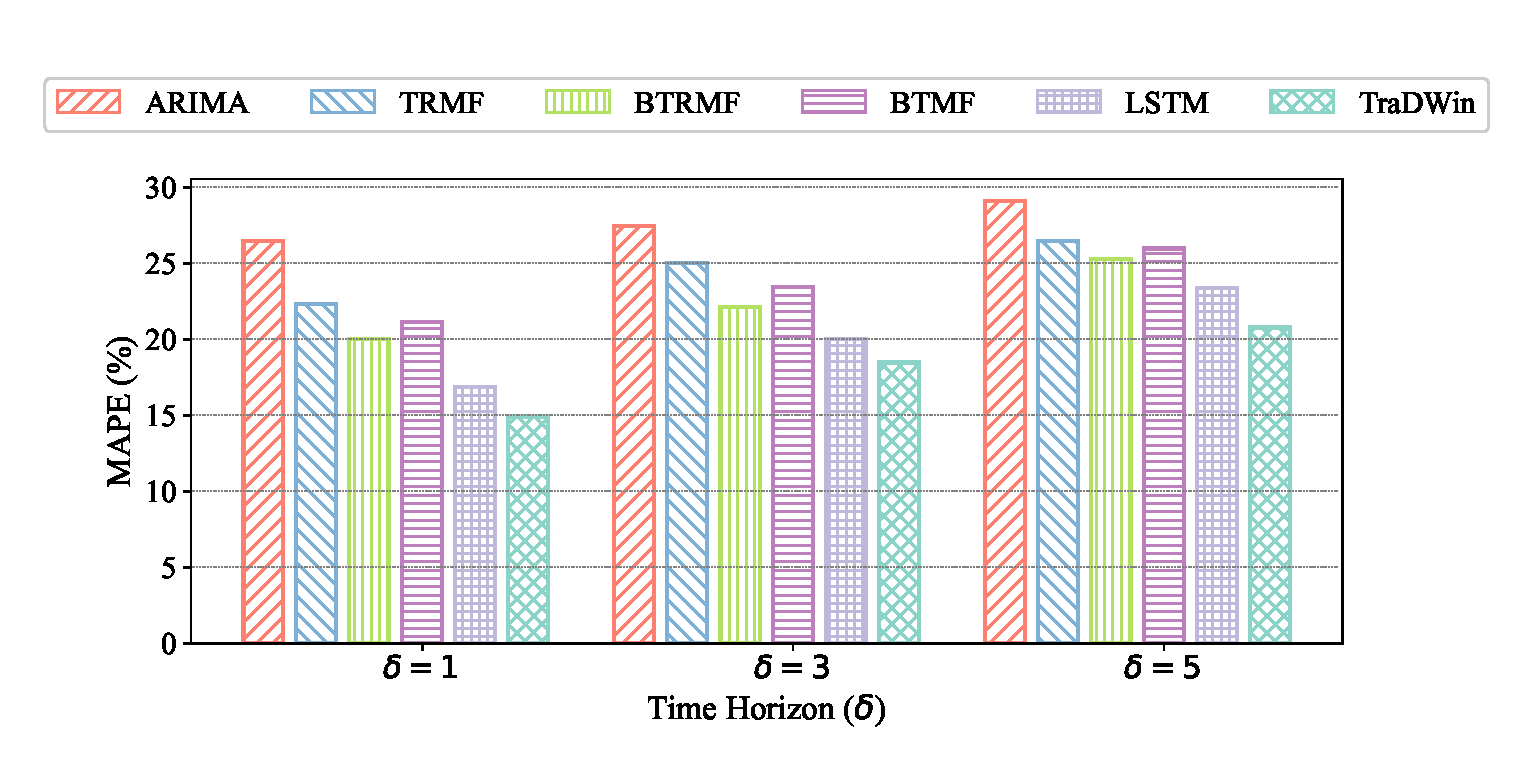
\includegraphics[width=0.9\textwidth]{mape_pred.eps}
    \caption{MAPE on prediction task for different deltas (timesteps to predict ahead)}
    \label{fig:mape_pred}
\end{figure*}

\begin{figure*}[]
    \centering
    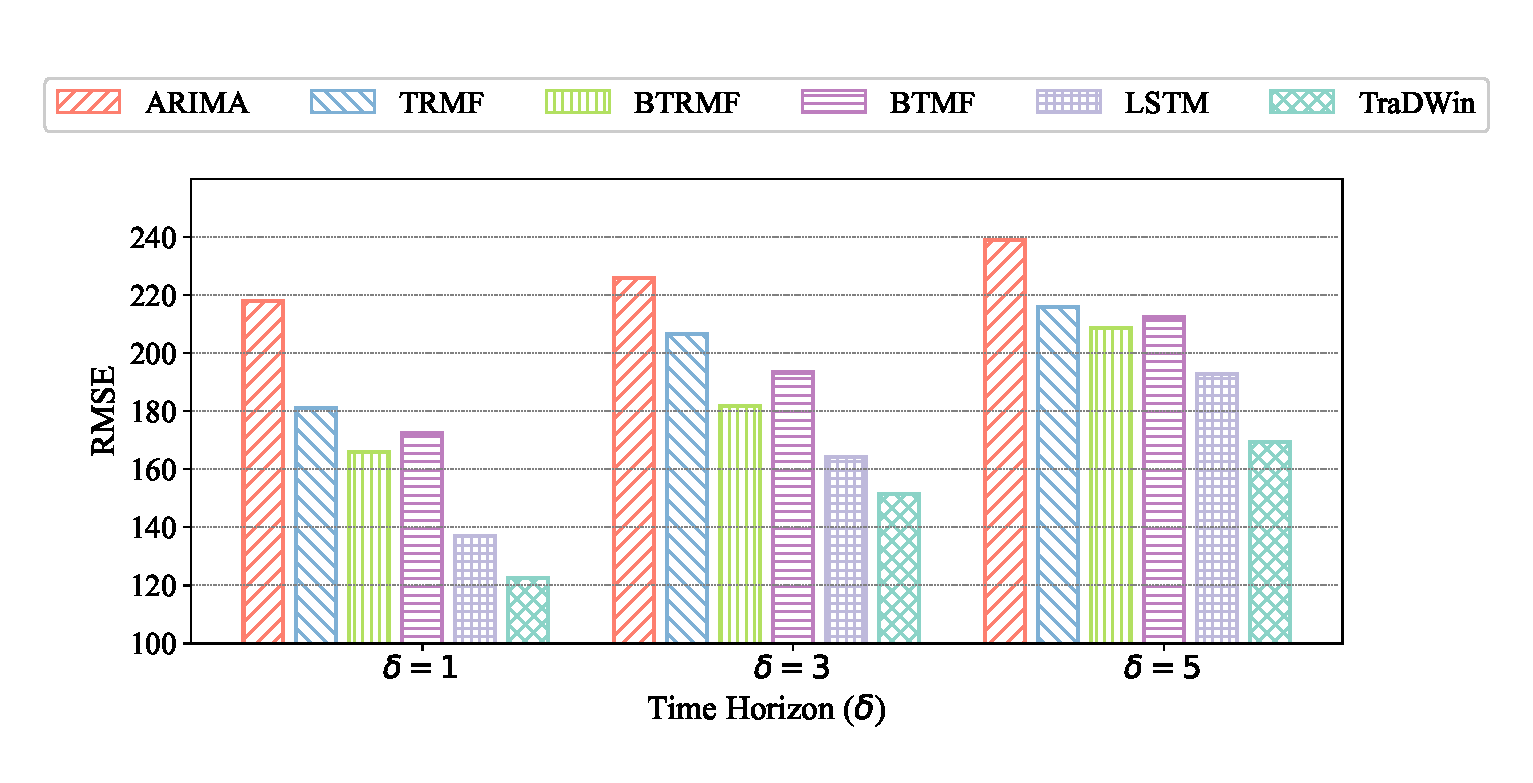
\includegraphics[width=0.9\textwidth]{rmse_pred.eps}
    \caption{RMSE on prediction task for different deltas (timesteps to predict ahead)}
    \label{fig:rmse_pred}
\end{figure*}

We evaluated the performance of our model on different tasks and compared them with other popular models used in the domain. For the prediction task, we tested the models for predicting traffic volumes at the next timestep, i.e., the forecasting $\delta = 1$, at the third timestep, i.e., $\delta = 3$ and the fifth timestep in future, i.e., $\delta = 5$. This scenario of predicting the next time step requires a mask consisting of all the $T_{n+1}$ values missing, i.e., 0. We prepare a mask similarly for other time horizons. Thus, prediction here is treated as a strict MNAR (Missing Not At Random) subcategory of imputation.

The MAPE and RMSE plots of prediction task on different horizons is shown in Fig. \ref{fig:mape_pred} and Fig. \ref{fig:rmse_pred} respectively. We observer that in general, as the $\delta$ i.e. the time horizon to predict in future, increases, both metrics worsen with MAPE falling 5-10\% from $\delta=1$ to $\delta=3$, i.e., we see a stronger short term accuracy but face some challenges with long-term prediction, across all models. This trend is common in time-series forecasting, where predictive accuracy decreases as the prediction horizon extends. The primary reasons for this decline include the increasing uncertainty and the influence of unpredictable external factors, such as accidents or weather changes. We see that ARIMA performs worst, which is to be expected since its the simplest of mathematical models among the baselines we consider. The other matrix factorization and Bayesian models like TRMF, BTRMF and BTMF perform better but given that they are stricly mathematical models, they (i) fail to capture the intricate traffic dynamics that a deep learning model can, and (ii) use only the timeseries traffic data and not the graph topology and external factors that our model considers like weather etc. Finally, we see that LSTMs are close with slightly (2-3\%) worse performance which could be attributed to lack of knowledge of graph topology that we incorporate in our model through $Node2Vec$.

\begin{figure*}[]
  \centering
  \begin{subfigure}{0.5\textwidth}
    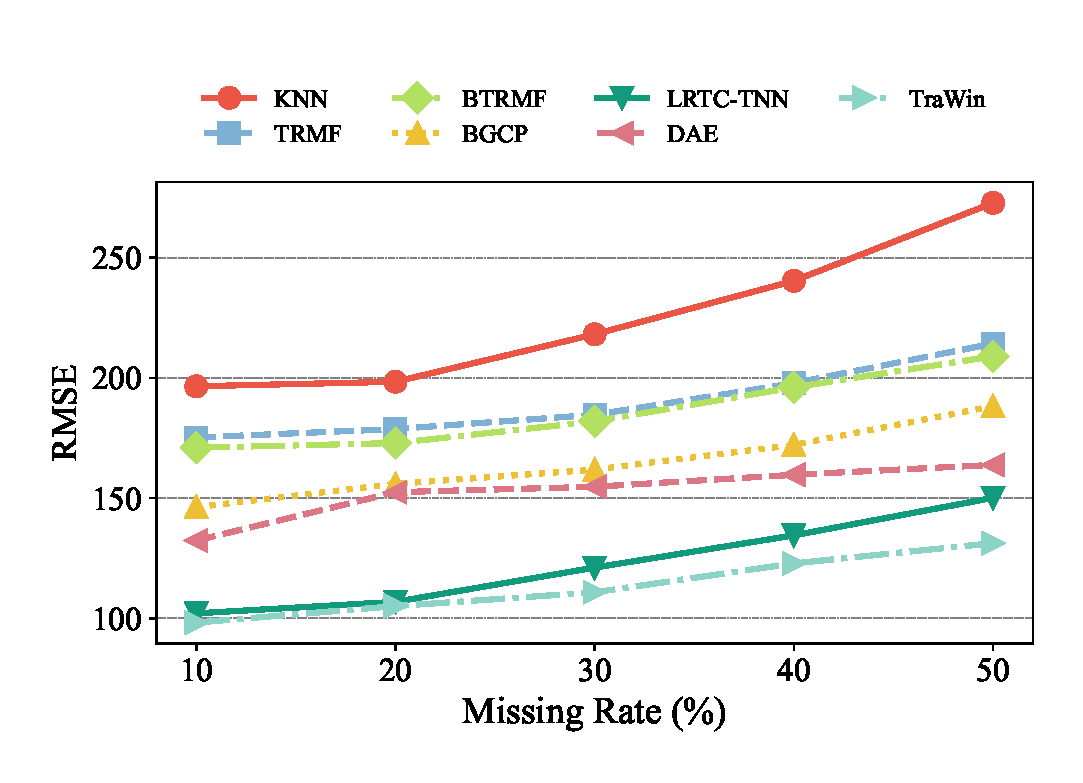
\includegraphics[width=\linewidth]{rmse_imput.eps}
    \caption{RMSE of different models on imputation task}
    \label{fig:mape_imput}
  \end{subfigure}%
  \begin{subfigure}{0.5\textwidth}
    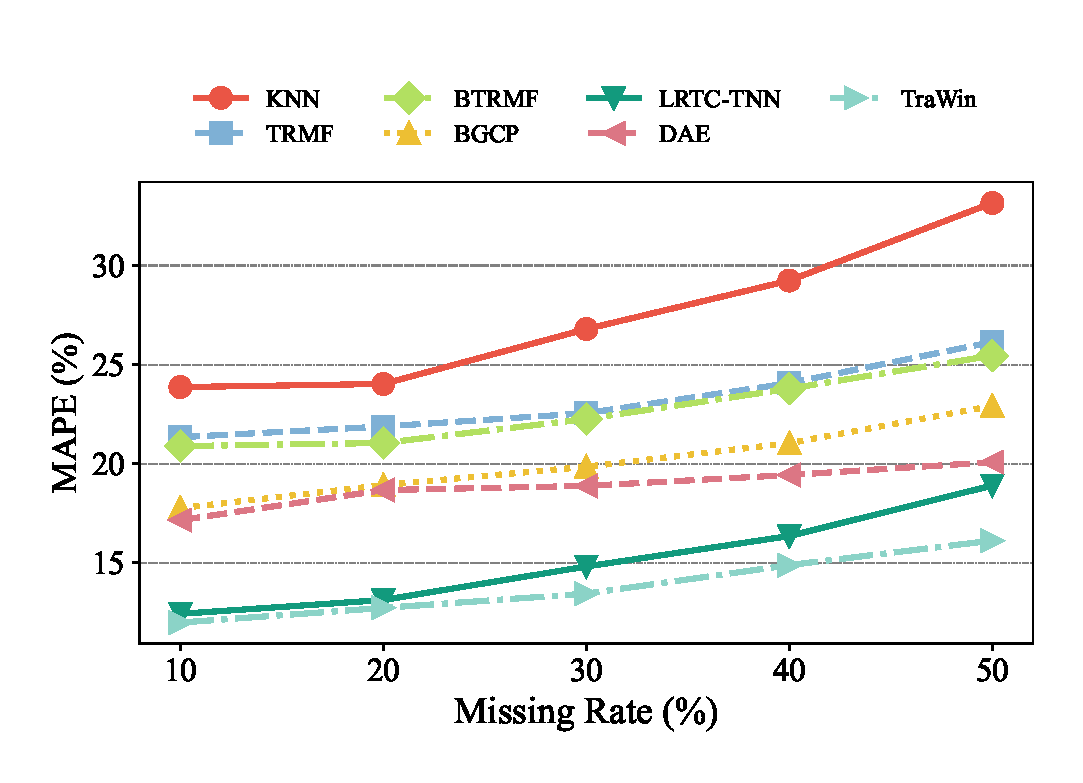
\includegraphics[width=\linewidth]{mape_imput.eps}
    \caption{MAPE of different models on imputation task}
    \label{fig:rmse_imput}
  \end{subfigure}
  \caption{Imputation comparison for different missing rates}
  \label{fig:imput}
\end{figure*}

Next, we evaluate performance on the imptation task. For this task, we have considered the MCAR (Missing Completely At Random) distribution and compare the models at five missing rates of $10\%$, $20\%$, $30\%$, $40\%$ and $50\%$. The perfomance of different models measured using MAPE and RMSE is shown in Fig. \ref{fig:imput}. We see that the conventional methods like KNN, perform poorly to more specialised approaches, which is to be expected since KNN is not enough to capture the intricate traffic dynamics. The matrix factorisation and Bayesian methods which are TRMF, BTRMF and BGCP work slightly better, with deep learning methods like DAE following ahead, though since they deal with only traffic data timeseries with no information on topology they have a 8-13\% worse off performane than out model. Tensor completion based model like LRTC-TNN is close to our \name in for low missing rates, but we see that it does not scale as well with increasing missing rate, possibly because too much data is lost for reliable tensor completion which a deep learning model can still handle, due to being able to learn more complex relationships in data and having knowledge of graph topology and other external factors. Moreover, it is worth nothing that LRTC-TNN is a MCAR imputer and not applicable to task (iii) so not generalised enough for our usecase. For all models, we see that the accuracy of imputations decreases with higher missing rates due to the reduced amount of contextual information available. This is a common challenge in data imputation, where fewer data points make it harder to discern underlying patterns accurately. 


\begin{figure}[t]
    \centering
    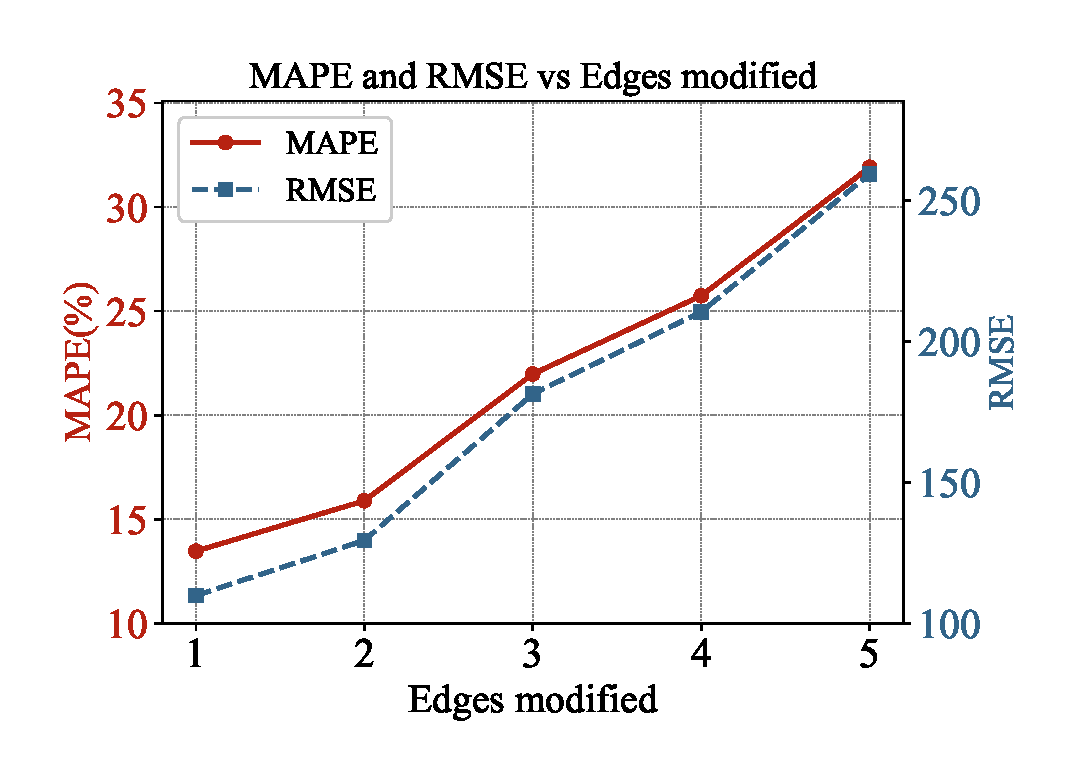
\includegraphics[width=\linewidth]{modif.eps}
    \caption{MAPE and RMSE on re-assignment task vs number of edges modified}
    \label{fig:edge_modif}
\end{figure}

We also observe that \name performs worse on task (i) than task (ii) by around 4\%. One primary reason for this, as we suspect, could be that GAIN that was originally designed for MCAR (Missing Completely At Random) imputation, does not generalise well to MNAR imputation scenarios. Another possible reason could be the subgraph-based computation method that we use, where nodes at the corners of the subgraph do not have adequate spatial and temporal information of their neighbors. Still, we observe that our model performs reasonably and delivers comparable results for being a generalized model.

Finally, on the re-assignment task, which is a new task that we address in our paper and is not conventionally seen in contemporary literature, we essentially train the model for MNAR (Missing Not At Random) imputation scenarios with the central node cluster missing. This effectively makes the model learn how to assign traffic to node clusters given neighbor node information. Based on this training task, we achieve a MAPE of $13.47\%$ and RMSE of $109.90$. Note that the other baselines considered for prediction and imputation are not applicable to this without changes to their model architecture so there is not comparison with contemporary models. Moreover, the de-facto way to solve this problem, as we have seen in our literature review, has been simulations like SUMO\cite{sumo} and Vissim\cite{vissim}. We too use those to compare and test our model on the TAPASCologne scenario using SUMO, which is a traffic simulation engine, with the configuration as described previously. The results of our model on this task are shown in Table. \ref{reassign_table}. We observe that the model achieves a MAPE of $13.47\%$ on Dublin SCATS dataset and $15.06\%$ on the TAPASCologne scenario, which demonstrates that the model can, with reasonable accuracy, learn to solve the traffic assignment problem on node clusters. Further, we tried to evaluate how our model's performance scales with number of modifications, i.e., how much can we alter the original graph such that the model is still viable to use for re-assignment. In Fig. 7, we show a comparison of MAPE and RMSE with number of edges modified. We see that performance declines steadily from $13.47\%$ at $1$ change to $31.91\%$ at 5 changes. So, altering more of graph leads to decline in performance, with drop being significant and sharp after $3$ modifications. A possible reason for this could be the mass masking strategy we use to train the model for task (iii). For 5 modifications, too many of the neighbouring nodes are masked leading to large loss of contextual information that knowledge of graph representation does not compensate enough. 


\begin{table}[]
\centering
\caption{Performance on re-assignment task (1 edge change) for different datasets}
\label{reassign_table}
\begin{tabular}{lcc}
\toprule
Dataset & MAPE (\%) & RMSE \\
\midrule
Dublin SCATS & 13.47 & 109.90 \\
TAPASCologne & 15.06 & 23.34 \\
\bottomrule
\end{tabular}
\end{table}